\section{Desarrollo}
	Los temas abordados en cada una de las conferencias son los siguientes:
	\paragraph{Primer Conferencia de Cibernética (1946, Marzo)}
	\begin{itemize}
		\item Redes neuronales simuladas emulando el cálculo de la lógica proposicional.
		\item Antropología y como las computadoras podrían aprender a aprender.
		\item Diferencias de percepción debido a daño cerebral.
		\item Ética derivada de la ciencia.
		\item Comportamiento repetitivo compulsivo
	\end{itemize}
	\paragraph{Segunda Conferencia de Cibernética (1946, Octubre)}
	\begin{itemize}
		\item Mecanismos teológicos en la sociedad.
		\item Conceptos de la psicología Gestalt.
		\item Comunicación mediante el tacto y químicos entre hormigas.
	\end{itemize}
	\paragraph{Tercera Conferencia de Cibernética (1947, Marzo)}
	\begin{itemize}
		\item Psicología de niños.
	\end{itemize}
	\paragraph{Cuarta Conferencia de Cibernética (1947, Octubre)}
	\begin{itemize}
		\item La perspectiva de la psicología.
		\item Aproximaciones analógicas y digitales de modelos psicológicos.
	\end{itemize}
	\paragraph{Quinta Conferencia de Cibernética (1948, Marzo)}
	\begin{itemize}
		\item Formación de la I en el lenguaje.
		\item Modelos formales aplicados al picoteo de los pollos.
	\end{itemize}
	\paragraph{Sexta Conferencia de Cibernética (1949, Marzo)}
	\begin{itemize}
		\item Memoria.
		\item ¿Tenemos neuronas y conexiones suficientes para el total de las capacidades humanas?
		\item Colaboración entre física y psicología.
	\end{itemize}
	\paragraph{Séptima Conferencia de Cibernética (1950, Marzo)}
	\begin{itemize}
		\item Interpretación analógica y digital de la mente.
		\item Lenguaje y teoría de la información.
		\item Lenguaje, símbolos y neurosis.
		\item Comprensión de las comunicaciones verbales.
		\item Análisis formal de la redundancia semántica en el inglés impreso.
	\end{itemize}
	\paragraph{Octava Conferencia de Cibernética (1951, Marzo)}
	\begin{itemize}
		\item Información como semántica.
		\item ¿Los autómatas pueden adaptarse a la lógica deductiva?
		\item Teoría de decisiones.
		\item Dinámica de grupos pequeños y comunicaciones de grupo.
		\item La aplicabilidad de la teoría de juegos a las motivaciones físicas.
		\item El tipo de lenguaje necesario para analizar el lenguaje.
		\item Comportamiento puro vs comunicación verdadera.
		\item ¿La psiquiatría es una ciencia?
		\item ¿Puede un evento mental que crear memoria ser inconsciente?
	\end{itemize}
	\paragraph{Novena Conferencia de Cibernética (1952, Marzo)}
	\begin{itemize}
		\item La relación de la neuropsicología con la resolución de problemas en la filosofía y epistemología.
		\item La relación de la Cibernética a un micro nivel con la biomedicina y los procesos celulares.
		\item La complejidad de los organismos con una función de la información.
		\item Humor, comunicaciones y paradojas.
		\item ¿Los autómatas ajedrecisticos necesitan ser aleatorios para poder vencer a los humanos?
		\item Homeostasis y aprendizaje.
	\end{itemize}
	\paragraph{Décima Conferencia de Cibernética (1953, Marzo)}
	\begin{itemize}
		\item Estudios de la actividad en el cerebro.
		\item Información semántica y sus medidas.
		\item Significado en el lenguaje y como es este adquirido.
		\item Como los mecanismos neuronales puede reconocer formas y acordes musicales.
	\end{itemize}



	% \begin{figure}[H]
	% 	\begin{center}
	% 		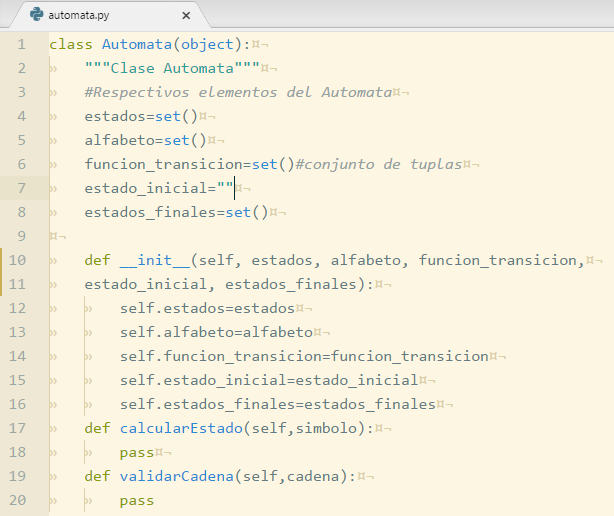
\includegraphics[width=15cm, height=12cm]{img/automata.png}
	% 		\caption{automata.py}
	% 		\label{fig:tablas}
	% 	\end{center}
	% \end{figure}